%%%%%%%%%%%%%%%%%%%%%%%%%%%%%%%%%%%%%%%%%
% Journal Article
% LaTeX Template
% Version 1.4 (15/5/16)
%
% This template has been downloaded from:
% http://www.LaTeXTemplates.com
%
% Original author:
% Frits Wenneker (http://www.howtotex.com) with extensive modifications by
% Vel (vel@LaTeXTemplates.com)
%
% License:
% CC BY-NC-SA 3.0 (http://creativecommons.org/licenses/by-nc-sa/3.0/)
%
%%%%%%%%%%%%%%%%%%%%%%%%%%%%%%%%%%%%%%%%%

%----------------------------------------------------------------------------------------
%	PACKAGES AND OTHER DOCUMENT CONFIGURATIONS
%----------------------------------------------------------------------------------------

\documentclass[twoside]{article}

\usepackage{blindtext} % Package to generate dummy text throughout this template 

\usepackage[sc]{mathpazo} % Use the Palatino font
\usepackage[T1]{fontenc} % Use 8-bit encoding that has 256 glyphs
\linespread{1.05} % Line spacing - Palatino needs more space between lines
\usepackage{microtype} % Slightly tweak font spacing for aesthetics

\usepackage[english]{babel} % Language hyphenation and typographical rules

\usepackage{parskip}

\usepackage[hmarginratio=1:1,top=32mm,columnsep=20pt]{geometry} % Document margins
\usepackage[hang, small,labelfont=bf,up,textfont=it,up]{caption} % Custom captions under/above floats in tables or figures
\usepackage{booktabs} % Horizontal rules in tables

\usepackage{lettrine} % The lettrine is the first enlarged letter at the beginning of the text

\usepackage{enumitem} % Customized lists
\setlist[itemize]{noitemsep} % Make itemize lists more compact

\usepackage{abstract} % Allows abstract customization
\renewcommand{\abstractnamefont}{\normalfont\bfseries} % Set the "Abstract" text to bold
\renewcommand{\abstracttextfont}{\normalfont\small\itshape} % Set the abstract itself to small italic text

\usepackage{titlesec} % Allows customization of titles
\renewcommand\thesection{\Roman{section}} % Roman numerals for the sections
\renewcommand\thesubsection{\roman{subsection}} % roman numerals for subsections
\titleformat{\section}[block]{\large\scshape\centering}{\thesection.}{1em}{} % Change the look of the section titles
\titleformat{\subsection}[block]{\large}{\thesubsection.}{1em}{} % Change the look of the section titles

\usepackage{fancyhdr} % Headers and footers
\pagestyle{fancy} % All pages have headers and footers
\fancyhead{} % Blank out the default header
\fancyfoot{} % Blank out the default footer
\fancyhead[C]{ $\bullet$ Report group 10 $\bullet$ } % Custom header text
\fancyfoot[RO,LE]{\thepage} % Custom footer text

\usepackage{titling} % Customizing the title section

% My packages (not template)
\usepackage{hyperref} % For hyperlinks in the PDF
%\usepackage{amsmath}
\usepackage{amssymb}
\usepackage{authblk}
\usepackage{graphicx}
\graphicspath{ {figures_report/} }

% From mortens LaTex file:
\usepackage{amsfonts, amssymb, amsmath}
\newcommand{\md}{\mathrm{d}}
\newcommand{\e}[1]{\times 10^{#1}}
\newcommand{\bra}[1]{\langle #1 |}
\newcommand{\ket}[1]{| #1 \rangle}
\newcommand{\braket}[2]{\langle #1 | #2 \rangle}
\renewcommand{\vec}[1]{\mathbf{#1}}
\newcommand{\gvec}[1]{\boldsymbol{#1}}
\newcommand{\dr}{\, \mathrm d^3 \vec r}
\newcommand{\dk}{\, \mathrm d^3 \vec k}

\usepackage{simpler-wick}

\usepackage{listings}
\usepackage{color}
 
\definecolor{codegreen}{rgb}{0,0.6,0}
\definecolor{codegray}{rgb}{0.5,0.5,0.5}
\definecolor{codepurple}{rgb}{0.58,0,0.82}
\definecolor{backcolour}{rgb}{0.95,0.95,0.92}
 
\lstdefinestyle{mystyle}{
    backgroundcolor=\color{backcolour},   
    commentstyle=\color{codegreen},
    keywordstyle=\color{magenta},
    numberstyle=\tiny\color{codegray},
    stringstyle=\color{codepurple},
    basicstyle=\footnotesize,
    breakatwhitespace=false,         
    breaklines=true,                 
    captionpos=b,                    
    keepspaces=true,                 
    numbers=left,                    
    numbersep=5pt,                  
    showspaces=false,                
    showstringspaces=false,
    showtabs=false,                  
    tabsize=2
}
 
\lstset{style=mystyle}
\renewcommand{\lstlistingname}{Code}

\usepackage{cancel}
\usepackage{tcolorbox} %to have boxes w color around text and math mode

\usepackage{footmisc}

%----------------------------------------------------------------------------------------
%	TITLE SECTION
%----------------------------------------------------------------------------------------

\setlength{\droptitle}{-4\baselineskip} % Move the title up

\pretitle{\begin{center}\Huge\bfseries} % Article title formatting
\posttitle{\end{center}} % Article title closing formatting
\title{Building a Shell Model Code Using the Pairing Model and NuShellX as Benchmark results} % Article title

%Old title: Building a Shell Model Code: The Pairing Model and the sd-Shell (and comparing results with NuShellX)

%another title: Using the Pairing Model and NuShellX to build a Shell-Model Code

\author[1]{ \textsc{Gianluca Salvioni} \footnote{Need credits for this report.}}
\author[2]{ \textsc{Ina K. B. Kullmann} *}
\author[3]{ \textsc{Matthew Shelley}}
\author[4]{ \textsc{Gilho Ahn}}

\affil[1]{Department of Physics, University of Jyv\"{a}skyl\"{a},  {\textit {\href{mailto:gianlucasalvioni@gmail.com}{gianlucasalvioni@gmail.com} }}}

\affil[2]{Department of Physics, University of Oslo,  {\textit {\ \href{mailto:i.k.b.kullmann@fys.uio.no}{i.k.b.kullmann@fys.uio.no} }}}

\affil[3] {Department of Physics, University of York, \textit {\href{mailto:mges501@york.ac.uk}{mges501@york.ac.uk} }}

\affil[4] {Department of Physics, National University of Athens, \textit {\href{mailto:gilahn@phys.uoa.gr}{gilahn@phys.uoa.gr} }}


% another way of doing the authors:
%\author{%
%\textsc{Gianluca Salvioni, Matthew Shelley, Gilho Ahn}\thanks{A thank you} \\[1ex]
%\normalsize University of Oslo \\ % Your institution
%\normalsize \href{mailto:i.k.b.kullmann@fys.uio.no}{i.k.b.kullmann@fys.uio.no} % Your email address
%\and % Uncomment if 2 authors are required, duplicate these 4 lines if more
%\textsc{Ina K. B. Kullmann}\thanks{Corresponding author} \\[1ex] % Second author's name
%\normalsize University of Oslo \\ % Your institution
%\normalsize \href{mailto:i.k.b.kullmann@fys.uio.no}{i.k.b.kullmann@fys.uio.no} % Your email address
%}



\date{\today} % Leave empty to omit a date

\renewcommand{\maketitlehookd}{%
\begin{abstract}
In this report we outline the steps we made to create a simple shell-model code starting from scratch. At first we face the pairing problem, for which we calculate an analytical solution and build a numerical implementation coded in the programming language Python.\\
In parallel we practice with a state-of-art code NushellX, to understand the important features of the Configuration Interaction method and the information we can gain from this to study nuclear structure properties.\\
From the skeleton of the pairing code, we construct a simple shell model code that can perform calculations in 1s0d shell model space for 1 up to 12 valence neutrons (from $^{17}$O to $^{28}$O). The energy levels obtained with our shell model code for the Oxygen isotopes are exactly equivalent to the results calculated with NushellX.
%We have first implemented the pairing model which have a analytical solution (to benchmark the code). Then implemented the sd shell ---> more general shell-model program that allows you to study general nuclear structure problems.

%developing our own shell-model code that can perform shell-model studies of the oxygen isotopes using standard effective interactions (provided by us) using as example the 1s0d shell as model space.

%We have also used the NushellX code in order to perform more advanced shell-model studies and compare the results obtained with your own shell-model code to those of NushellX

%and found that.....results... (abstract should not be longer than this ish)
\end{abstract}
}

%----------------------------------------------------------------------------------------

\begin{document}

% Print the title
\maketitle
\tableofcontents


%----------------------------------------------------------------------------------------
%	ARTICLE CONTENTS
%----------------------------------------------------------------------------------------

\section{Introduction}

%\lettrine[nindent=0em,lines=3]{L} orem ipsum dolor sit amet, consectetur adipiscing elit.
%\blindtext % Dummy text
%
%\blindtext % Dummy text

% WHY and WHERE USEFUL
The atomic nucleus is a complex system. 
It has the dimension of few fm (10$^{-15}$m) so the structure of the nucleus is regulated by quantum mechanics. 
We are interested in describing the low-energy scale that determine the nuclear configuration. Even though  the fundamental particles that form a nucleus are quarks and gluons, the degrees of freedom we explore are protons and neutrons. The number of nucleons can be between one and a couple of hundreds, requiring a many-body treatment.\\ 
The sub-atomic system is one of the most attractive laboratories to study physics. Three different natural forces play an active role in the nucleus: the strong, electromagnetic and weak interaction. 
The Coulomb force acting among protons and the electromagnetic transitions are manifestations of the electromagnetic force.
Beta decays are an example of weak interactions.
The strong force keeps the nucleons together in a bound state, but this interaction is not yet fully understood. There exist no complete equation for the strong force. Comparing theoretical results of effective interactions with available experimental data help us investigate the importance of the different terms in the interaction models.

One of the aims of nuclear physics is to explain the properties of all the observed nuclei. The properties of the nuclei are also called observables and include the binding energy (mass), spin, radius, deformation, electromagnetic moments as well as life-time, excitation energies, electromagnetic transitions, decays, particle emissions and so on. 

%-(Look at the TALENT proposal) \\

% COMPARE METHODS \\
\begin{figure}[ht]
\centering
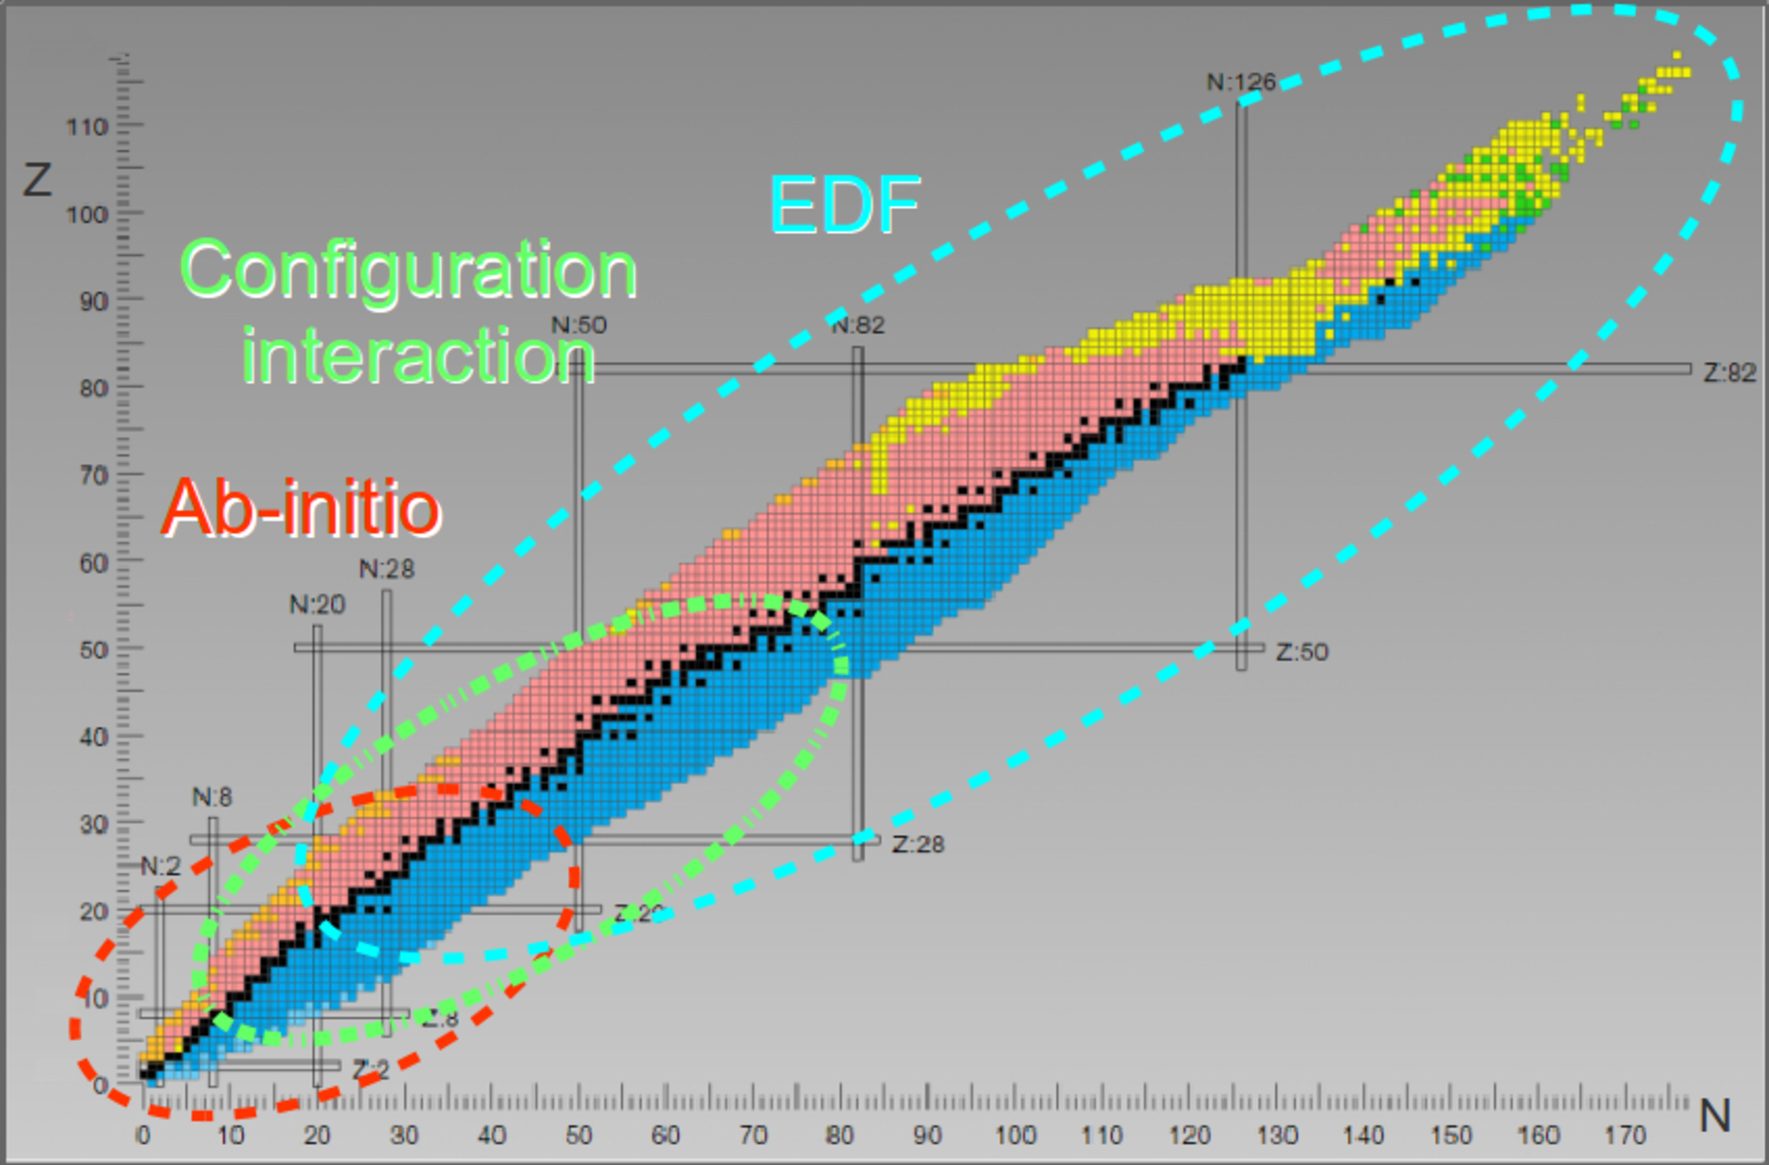
\includegraphics[width=0.8\textwidth]{nuclear_chart.pdf}
\caption{In this nuclear chart the known nuclei are plot according to the neutron number $N$ (x-axis) and proton number $Z$ (y-axis). The domain of Ab-initio, Configuration Interaction and Energy Density Functional  models are pictured. The nuclei represented in black are the stable ones.}
\label{fig: nuclear_chart}
\end{figure}
Another goal is to predict the limits of the possible bound systems (driplines). The nuclear chart can be described by three different theoretical models, as shown in Figure \ref{fig: nuclear_chart}.
Light nuclei, $A \lesssim 20$ is the playground of Ab-initio methods where an interaction derived by first principles (close to quantum chromodinamics) are applied and all the nucleons are taken into account. Medium mass nuclei, $ 16 \lesssim A \lesssim 132$ can be studied by Configuration Interaction theory, also known as shell-models. Truncation of the model space is key to study large systems with shell-models due to limitations in computing resources. Heavy nuclei are usually described by Energy Density Functionals that reduce the volume of information needed. The the price for this information reduction is that mainly ground state properties can be calculated.

% ANTICIPATION OF THE CONTENTS
In this report we consider the Configuration Interaction method. In Sec.\ref{sec:pair} we start to study a basic pairing model to practise with the second quantization formalism and the building block of the shell-model. We will obtain analytical results that we implement in a Python code to be used as benchmark for our own shell model code later.

In Sec.\ref{sec: NushellX} we learn how to use state-of-the-art Configuration Interaction code NushellX and perform calculations of the Oxygen isotopic chain in the $sd$-model space.

We extend our Python code in Sec.\ref{sec:ourcode} to describe, through full the Configuration Interaction method, neutrons in the $sd$-model space with the goal to study the simple isotopic chain $^{17}$O-$^{28}$O. We develop our shell model code beyond the pairing model and compare our energy levels to calculations done with NuShellX.

Further possible developments are discussed in Sec.\ref{sec:discussion} and finally our achievements are summarized in Sec.\ref{sec:summary}.
 
%------------------------------------------------
\newpage

\section{The pairing problem}
\label{sec:pair} 

The starting point for our shell-model code is a pairing model: the system consists of fermions combined together in pairs of two, one with spin up and one with spin down. In this section we will calculate the analytic results of the pairing model that was used to validate our shell-model code at an early stage in the development. The assumption in this model is that the 'breaking of pairs' is not allowed, i.e. the pairs of particles will always be coupled together, forming states with $J$=0. Of consequences the excited states are obtained from the excitation of two particles at the same time. 

%we could have a subsection here instead of a paragraph..?

\paragraph{The theory of the pairing model.} The physics of this system can be described by an Hamiltonian $\hat H$ consisting of an unperturbed one-body operator $\hat H_0$ and a two-body pertubation $\hat V $ defined as 'pairing potential': $\hat H = \hat H_0 + \hat V$. In second quantization we can write:

\begin{equation}
\hat H_0 =  \sum_{p,\sigma} (\epsilon_p-1) \hat a_{p\sigma}^\dagger \hat a_{p\sigma},
\label{eq:H_0}
\end{equation}

\begin{equation}
\hat V = -\frac{1}{2} g \sum_{p,q} \hat a_{p+}^\dagger \hat a_{p-}^\dagger \hat a_{q-} \hat a_{q+} ,\label{eq:V}
\end{equation}
where the fermion creation and annihilation operators are given by $\hat a_{p}^\dagger$ and $\hat a_{q}$ respectively and $pqrs$ represent all possible single-particle quantum numbers.

The single-particle states $\vert p \rangle$ are chosen as eigenfunctions of the one-particle operator $\hat{h}_0$, then the Hamiltonian $H$ acts in turn on various many-body Slater determinants constructed from the single-basis defined by the one-body operator $\hat{h}_0$.

The two-body pairing operator $\hat{V}$ is:
\begin{equation}
\langle q_+ q_- \vert \hat{V} \vert s_+s_- \rangle = -g
\end{equation}
where it is explicitly shown that for a given matrix element $\langle pq \vert \hat{V} \vert rs \rangle$ the states $p$ and $q$ (or $r$ and $s$) must have opposite spin ($\sigma=\pm 1$). $g$ is the (constant) strenght of the pairing interaction.

Using the formalism of second-quantization, the rules of anticommutation for fermions and the products of commutating and anticommutating operators it can be shown that $\hat{H}_0$ and $\hat{V}$ commute with the spin projection $\hat{J}_z$ and the total spin $\hat{J}^2$. This means that $H$ can be diagonalized in separated blocks. And due to the 'no-broken pair' assumption, only $J = 0$ are allowed.


\paragraph{Constructing the Hamiltonian matrix.}

We are now interested to consider a system consisting of only four particles to calculate its exact analytic solution as benchmark for our shell-model code. The single-particle space is constructed by the four lowest levels with single-particle level energies $\epsilon_p = 1, 2, 3, 4$. Every level $\epsilon_p$ contains two particles, one with spin up $\vert p+ \rangle$ and one with spin down $\vert p- \rangle$. 

The possible Slater determinants that we can build are 6:
\begin{align*}
\ket{\Phi_0} &= \hat a_{2+}^\dagger \hat a_{2-}^\dagger \hat a_{1+}^\dagger \hat a_{1-}^\dagger \ket{0}  \\
%
\ket{\Phi_1} &= \hat a_{3+}^\dagger \hat a_{3-}^\dagger \hat a_{1+}^\dagger \hat a_{1-}^\dagger \ket{0}  \\
%
\ket{\Phi_2} &= \hat a_{4+}^\dagger \hat a_{4-}^\dagger \hat a_{1+}^\dagger \hat a_{1-}^\dagger \ket{0}  \\
%
\ket{\Phi_3} &= \hat a_{3+}^\dagger \hat a_{3-}^\dagger \hat a_{2+}^\dagger \hat a_{2-}^\dagger \ket{0}  \\
%
\ket{\Phi_4} &= \hat a_{4+}^\dagger \hat a_{4-}^\dagger \hat a_{2+}^\dagger \hat a_{2-}^\dagger \ket{0}  \\
%
\ket{\Phi_5} &= \hat a_{4+}^\dagger \hat a_{4-}^\dagger \hat a_{3+}^\dagger \hat a_{3-}^\dagger \ket{0} , \\
\end{align*}

from which we can construct the basis for the Hamiltonian matrix:
\[ \ket{\Phi_0} = \begin{pmatrix} 1 \\ 0 \\ 0 \\ 0 \\ 0 \\ 0 \end{pmatrix}, \quad
\ket{\Phi_1} = \begin{pmatrix} 0 \\ 1 \\ 0 \\ 0 \\ 0 \\ 0 \end{pmatrix}, \quad \cdots \quad
\ket{\Phi_5} = \begin{pmatrix} 0 \\ 0 \\ 0 \\ 0 \\ 0 \\ 1 \end{pmatrix}. \]

The matrix elements $H_{ij}=\bra{\Phi_i} \hat H \ket{\Phi_j}$ \footnote{We use the label 0 to indicate the Slater determinants with the 4 particles in the lowest states, then the first row first column matrix element is $H_{00}$....} are obtained using the Hamiltonian of Eq.~\eqref{eq:H_0}, the Slater determinants and the Wick-theorem. $\hat H_0$ acts only on the diagonal and results in terms proportional with $(\epsilon_p-1)$. The interaction will excite or deexcite a pair of particles from level $q$ to level $p$. \\Using the Wick-theorem, we notice that only the Slater determinants that differ for maximum a pair can interact among them through the pairing potential:
\begin{eqnarray}\label{Vwick}
\bra{\Phi_i} \hat V \ket{\Phi_j} &=&  \bra{0} \hat a_{i_1-} \hat a_{i_1+} \hat a_{i_2-} \hat a_{i_2+} \left[ -\frac{1}{2} g \sum_{p,q} \hat a_{p+}^\dagger \hat a_{p-}^\dagger \hat a_{q-} \hat a_{q+} \right] \hat a_{j_2+}^\dagger \hat a_{j_2-}^\dagger \hat a_{j_1+}^\dagger \hat a_{j_1-}^\dagger \ket{0} \nonumber \\
&=& -\frac{1}{2} g  \left(\delta_{p, i_2} \delta_{q, j_2} \delta_{i_1,j_1} + 
\delta_{p, i_2} \delta_{q, j_1} \delta_{i_1,j_2} + 
\delta_{p, i_1} \delta_{q, j_2} \delta_{i_2,j_1} +
\delta_{p, i_1} \delta_{q, j_1} \delta_{i_2,j_2} \right) 
\end{eqnarray}

and Eq.(\ref{Vwick}) is not null only if at least one of $\delta_{i_1,j_1}, \delta_{i_1,j_2}, \delta_{i_2,j_1}$ or $\delta_{i_2,j_2}$ among bra and ket states is not zero.\\
For example the first term in Eq.(\ref{Vwick}) is obtained from the contractions

\begin{equation}
 \bra{0} \wick{  \c1{\hat a_{i_1-}} \c2{\hat a_{i_1+}} \c3{\hat a_{i_2-}} \c4{\hat a_{i_2+}} \c4{\hat a_{p+}^\dagger} \c3{\hat a_{p-}^\dagger} \c5{\hat a_{q-}} \c6{\hat a_{q+}} \c6{\hat a_{j_2+}^\dagger} \c5{\hat a_{j_2-}^\dagger} \c2{\hat a_{j_1+}^\dagger} \c1{\hat a_{j_1-}^\dagger}} \ket{0} = \delta_{p, i_2} \delta_{q, j_2} \delta_{i_1,j_1}. \nonumber
\end{equation}
 
 Explicitly, the matrix element $H_{00}$ is
\begin{eqnarray}
\bra{\Phi_0} \hat H \ket{\Phi_0} &=& \bra{0} \hat a_{1-} \hat a_{1+} \hat a_{2-} \hat a_{2+} \left[ \sum_{p,\sigma} (\epsilon_p-1) \hat a_{p\sigma}^\dagger \hat a_{p\sigma} \right] \hat a_{2+}^\dagger \hat a_{2-}^\dagger \hat a_{1+}^\dagger \hat a_{1-}^\dagger \ket{0} \nonumber \\
&+& \bra{0} \hat a_{1-} \hat a_{1+} \hat a_{2-} \hat a_{2+} \left[ -\frac{1}{2} g \sum_{p,q} \hat a_{p+}^\dagger \hat a_{p-}^\dagger \hat a_{q-} \hat a_{q+} \right] \hat a_{2+}^\dagger \hat a_{2-}^\dagger \hat a_{1+}^\dagger \hat a_{1-}^\dagger \ket{0} \nonumber \\
&=& 2 \cdot 0+2 \cdot (2-1)+ 2\cdot \left(-\frac{1}{2} g \right) = 2-g.
\end{eqnarray}

The Hamiltonian matrix becomes

\begin{equation}
\hat H = \begin{pmatrix}
2 - g & -g/2 & -g/2 & -g/2 & -g/2 & 0 \\
-g/2 & 4- g & -g/2 & -g/2 & 0 & -g/2 \\
-g/2 & -g/2 & 6 -g & 0 & -g/2 & -g/2 \\
-g/2 & -g/2 & 0 & 6 -g & -g/2 & -g/2 \\
-g/2 & 0 & -g/2 & -g/2 & 8 - g & -g/2 \\
0 & -g/2 & -g/2 & -g/2 & -g/2 & 10 - g \\
\end{pmatrix} .
\label{eq: analytic_H_matrix} 
\end{equation}

\begin{figure}[ht]
\centering
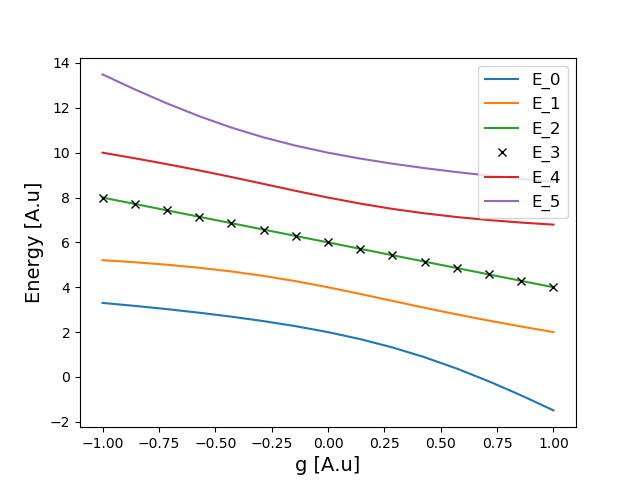
\includegraphics[width=0.8\textwidth]{eigval_vs_g.png}
\caption{The energy levels as a function of the strength $g$ for the analytic case of the pairing model. }
\label{fig: g_vs_eigval}
\end{figure}

In Figure \ref{fig: g_vs_eigval} we see the eigenvalues of the Hamiltonian matrix \eqref{eq: analytic_H_matrix} for the pairing model as a function of the strength $g \in [-1,1]$. \footnote{The diagonalization was done with \texttt{numpy}.}. We can observe that the pairing potential increases the gap among the energy levels $E\_i$, eigenvalues of Eq.(\ref{eq: analytic_H_matrix}). The case $g=1$, corresponding to a strong attractive pairing, produces the more stable system (lowest energy levels).

%------------------------------------------------
\newpage

\section{NuShellX}
\label{sec: NushellX}

NushellX is a code developed by W. D. M. Rae \cite{ref: nushellx} that provides an powerful tool for nuclear structure calculations. This shell-model code is capable of Hamiltonian matrix calculations with very large basis dimensions. With NuShellX one can obtain energies, eigenvectors and spectrosopic overlaps for low-lying states. Here we are interested in extract energies from NuShellX that will be used to benchmark our shell-model code in the development beyond the pairing model. 

%NuShellX uses $J$-scheme and $jj$-coupling. It is written in $pn$-formalism; it uses a J-coupled proton-neutron. % Is this written in the code documentation??? Because we can decide to use pn-interaction or isospin dependent interaction
NushellX is written in $pn$-formalism, i.e. the model space considers neutron and protons states separately, and couples them in $J$-scheme. The single-particle basis, the states for protons and neutrons are created separately. The code can consider $J$-scheme matrix dimensions of up to the order of a 100 million. To take advantage of many cores in modern computers, OpenMP for the Lanczos iterations is used. This way the code can handle quite large model spaces in a reasonable time on a laptop too.  

%The major disadvantage of NuShellX is that it is very easy to produce unrealistic or inappropriate results. 
Calculations in an infinite space are not possible and therefore some truncation is required. Ideally one would like to do calculations in the largest possible model spaces and one can argue that the best and most complete results are found with the largest model spaces. The major issue is that the computational time increases exponentially with model space size, so the wish for large model spaces are limited by the computational power and time available. When doing a calculation it may be useful to first truncate severely and quickly get a first crude result. Then one can later relax the truncations until the desired accuracy is reached. 

Another challenge when running shell model calculations is that the chosen interaction must be appropriate for the model space. A calculation in the full model space may be too computationally intensive in itself, but it may also be inappropriate for the interaction. To run a shell model calculation one have to make two major decisions: which interaction will we use, and which model space truncation? In NuShellX only subshell truncations can be made. We can only limit the number of valence particles (protons and neutrons separately) in a given orbital. %We cannot restrict the total number of nucleons in a given orbital since protons and neutrons are treated separately. 

\begin{figure}[ht]
\centering
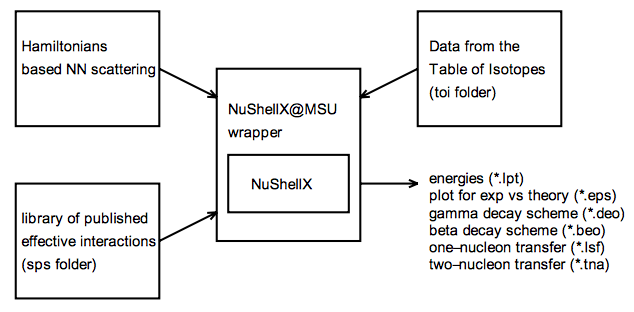
\includegraphics[width=0.8\textwidth]{nushellX_structure_from_ref.png}
\caption{Schematic layout of the NuShellX@MSU codes from Ref.\cite{ref: nushellx} }
\label{fig: nushellx_struct}
\end{figure}

\paragraph{Running a NuShellX calculation.} A set of wrapper codes called NuShellX@MSU is written by Alex Brown. These wrapper codes generates input for the NuShellX code and converts the output into tables and figures for energy levels, gamma decay and beta decay. In figure \ref{fig: nushellx_struct} we see the outline of the in- and output administered by the NuShellX@MSU wrapper code. When \texttt{shell} is run the user is asked to provide\footnote{not all options are given in this example, the input depend on the type of calculation done with NuShellX}:

\begin{itemize}
\item the batch file name
\item the model space name
\item restrictions / truncations
\item interaction name
\item number of protons and nucleons
\item min and max J and parity
\item extended functionalities
\end{itemize}

The NuShellX@MSU code provides the model spaces (\texttt{*.sp}) and hamiltonians (\texttt{*.int}) found in the \texttt{sps} folder. The file \texttt{label.dat} contains a list of available model space and hamiltonian combinations. For a more detailed description of how to run the NuShellX code see Ref.\cite{help_file}.

The extended functionality (called by the option \texttt{den}) make NushellX a powerful program to study atomic nuclei. This option makes it possible to calculate electromagnetic transitions, neutron and proton emission, beta decay as well as Hartree-Fock calculations in Energy Density Functional style. In this report we will only show the NuShellX calculations that will be used to benchmark our own shell model code. 

\paragraph{NuShellX results.} We calculated the excitation energies of the isotopes $^{17}$O to $^{28}$O using the $usdb$ effective interaction optimized for the 1s0d shells. In Figure \ref{expnushellx} the results for $^{18}$O and $^{20}$O is shown. The plot is generated by the NuShellX@MSU code, we see the theoretical results (left) and the the experimental available values (right) for each isotope. We observe that the agreement between theory and experiment is good, especially for the lowest excited states. 

\begin{figure}[h]
\begin{center}$
\begin{array}{c c}
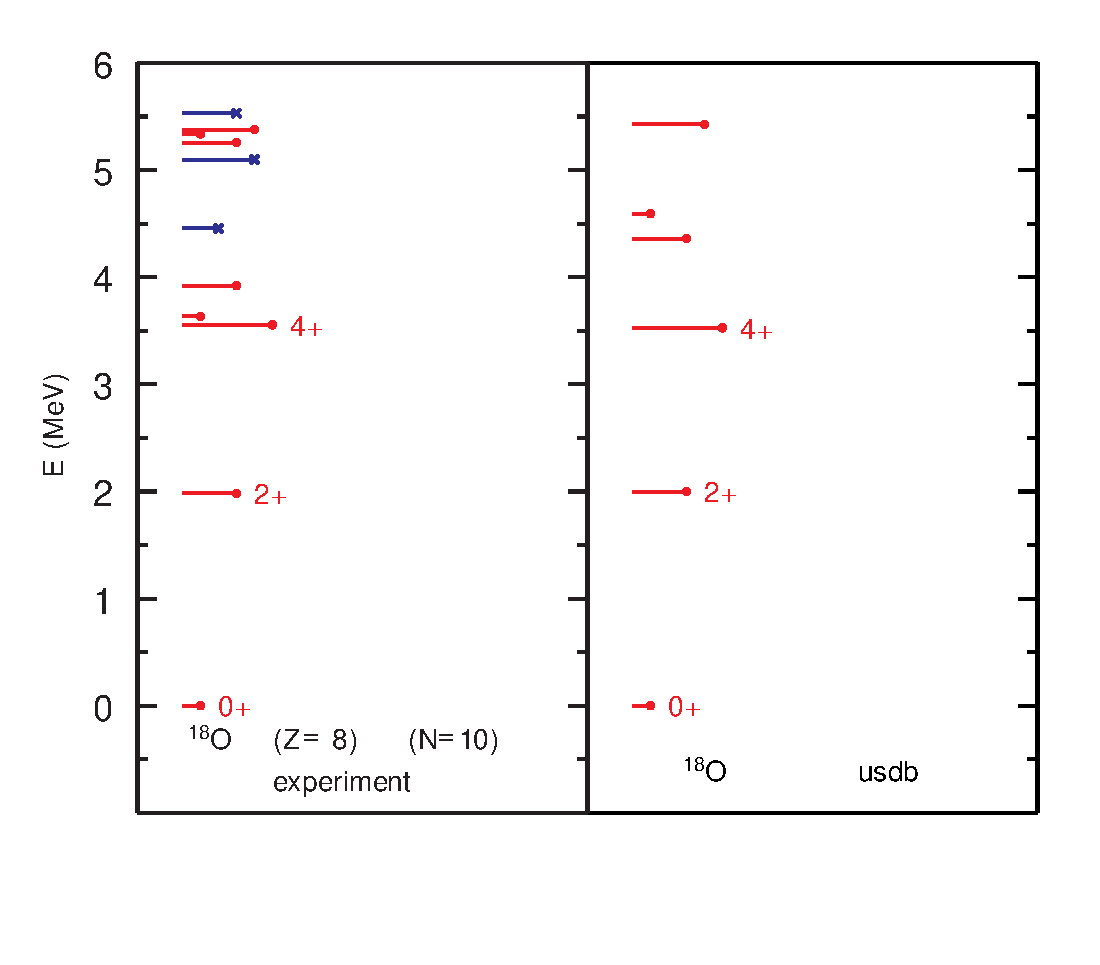
\includegraphics[scale=.4]{o_18b.eps} &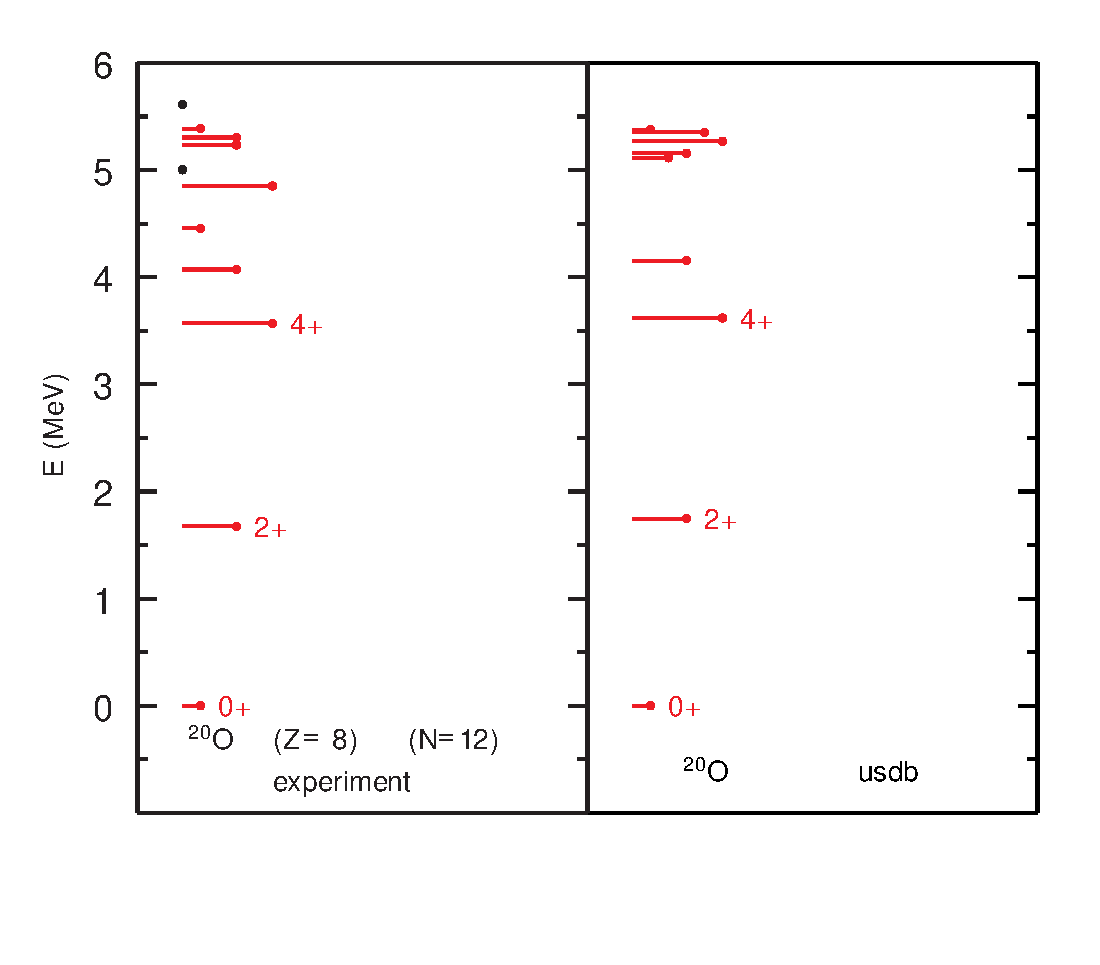
\includegraphics[scale=.4]{o_20b.eps} 
\end{array}$
\end{center}
\caption{ Example of calculation of the energy levels done with NushellX for $^{18}$O and $^{20}$O and their relative experimental values. The agreement is good especially for the lowest excited states.}
\label{expnushellx}
\end{figure}


%------------------------------------------------
\newpage

\section{Building our shell-model code}
\label{sec:ourcode}

Our goal is to describe the specific case of the $O$ isotopes within the $sd$ model space. In this section we will not describe the code of the pairing model in detail, we simply state that we are building on a working code that reproduce the results given in Sec.\ref{sec:pair}. From this we will extend our code to perform shell-model calculations. Our results will be directly compared and benchmarked to the same calculations performed with NushellX.

\subsection{The structure of the code}

We construct our shell-model code step by step, keeping in mind that we are interested in describing a system with $N$ particles in the valence space. The code is organized into blocks of code, or modules, stored in separate files that performs different tasks. The files needed to run the shell-model code is:
\begin{itemize}
\item \texttt{main.py}
\item \texttt{input\_func.py}
\item \texttt{create\_table\_files.py}
\item \texttt{read\_files.py}
\item \texttt{unit\_tests.py} 
\item \texttt{compare.py}
\item \texttt{ham.py} 
\end{itemize}
\smallskip

The \texttt{main.py} program runs the code and calls the functions in the other files. The structure of the \texttt{main.py} program is listed\footnote{We refer to this 'structure list' and its numbering later in the text (point ...).} below:

\begin{tcolorbox}
\begin{enumerate}
\item Import files (modules)
\item Ask user to provide input on the command line. The only inputs needed are \label{list: user_input}
\begin{itemize}
\item \texttt{N\_particles} - number of valence particles (neutrons) 
\item \texttt{case} - model space 'sd' (or 'pairing')
\item \texttt{g} - strenght of the pairing (needed only in 'pairing' case)
\end{itemize}
\item Read the single-particle basis \label{list: sp}
\item Create all the possible the Slater Determinants \label{list: SD}
\item Read and store the two-body matrix elements (tbme). In the case 'pairing', create all the non-zero pairing matrix elements according to the given strenght $g$. \label{list: tbme}
\item Build the total Hamiltonian matrix from the one- and two-body terms \label{list: build_ham}
\item Check (unit test) if the Hamiltonian for the pairing problem is correct. If not exit the program with an error message \label{list: unit_test}
\item Solve the diagonalization problem and print the eigenvalues and eigenvectors of the problem \label{list: diag_eigval_vec}
\end{enumerate}
\end{tcolorbox}

%NOT TRUE ANYMORE Before the basis, Slater determinants and the tbme are created the program checks, for each case if the file already exist. If the file containing for instance the basis do not exist the basis will be generated and saved to file before the code reads the file. If the file with the basis already exist the code will jump to reading the file. This way we avoid creating the (same) files every time the code is run. 

\smallskip

\noindent \textbf{To run the code} one simply type the following into the terminal
\begin{center}\texttt{python main.py}\end{center} 
and the program will interactively ask the user for input in the terminal (point \ref{list: user_input}). The user input function is implemented in such a way that the user is not allowed to provide unphysical input values. If invalid input is given the program provides an error message and asks the user to provide the input within the allowed type or interval. When the input is given the program runs and prints the results in the terminal.

\subsection{The model space and the Slater determinants}

%\paragraph{The model space.}
The single-particle states are the fundamental building blocks of the shell model, in fact they form the so called 'single-particle basis'. As indicated in the 'structure list' (point \ref{list: sp}), reading in the basis is the first step after the input is given. In our case we read the information of the single-particle levels from file. For example \texttt{sd\_shell.sp} contains the quantum number $n$,$l$,$2j$ and $2m_j$ together with their energy levels (eigenvalue of the single-particle Hamiltonian). This file was provided in the first part of the file \texttt{sdshellint.dat}\cite{file_link}. Looking at the energies we can notice a degeneration respect to the $m_j$ quantum number.


%\paragraph{The Slater determinats.} 
The next step in the 'structure list' is to create all the possible Slater Determinants (point \ref{list: SD}). A Slater determinant $\ket{\Phi_i}$ is a product of $N$ single-particle states that differ from each other (we are working with fermions and we need to satisfy the Pauli principle). The total number of Slater determinants which can be built with $N$ particles distributed among $i$ single-particle states is
\begin{equation}\label{binSD}
d=\left (\begin{array}{c} i \\ N\end{array} \right) =\frac{i!}{(i-N)!N!}. 
\end{equation}
The $N$-particle wave function, the solution of the Hamiltonian $H$ is a linear combination of the Slater determinants constructed inside the model space. In \texttt{create\_table\_files.py} we calculate all possible Slater determinats (see Code \ref{create_SD}) and store them in \texttt{sd\_SlaterD.sd}. We work in $m$-scheme and we do not impose any condition on the total $M= \sum m_j$.

\begin{lstlisting}[language=Python,label=create_SD,caption=The function \texttt{create\_SD\_perm} in the file \texttt{create\_table\_files.py} uses the Python function \texttt{itertools.combinations(,)} to create all the possible Slater determinants. In the case of the pairing model the Slater determinants are restricted to the ones with $\protect{M=0}$ and coupled pairs of single-particle states.]
import numpy as np
import itertools

def create_SD_perm(N_particles, nr_sp_states, sp_matrix, SD_filename, restrictions=''): 
    ...

    nr_sp_states = int(nr_sp_states)
    sp_list = []
    for i in range(1, nr_sp_states+1):
        sp_list.append(i)
    sp_tuple = tuple(sp_list)
    #print sp_tuple
    index = 0
    SD_list = []
    act_list = []
    for x in itertools.combinations(sp_tuple, N_particles):
        m_tot = 0
        for k in range (N_particles):
            m_tot = m_tot + sp_matrix[x[k]-1,4]
        #PAIRING CASE
        # only N_particles even is considered
        if restrictions == 'pair':
            if N_particles%2 == 0:
                pair_bool = 0
                # check that the single-particle states are in pairs
                for j in range (0,N_particles,2):
                    if np.array_equal(sp_matrix[x[j]-1,1:3], sp_matrix[x[j+1]-1,1:3]):
                        pair_bool = pair_bool 
                    else:
                        pair_bool = pair_bool +1
                # check that M=0 and pairs are coupled
                if m_tot == 0 and pair_bool == 0:
                    index +=1
                    SD_list.append(index)
                    SD_list.extend(list(x))
        #GENERAL CASE
        else:
            index +=1
            SD_list.append(index)
            SD_list.extend(list(x))
    
    nr_SD = index
    SD_array = np.array(SD_list)
    SD_states = SD_array.reshape(nr_SD,N_particles+1)
    ...

\end{lstlisting}

\subsection{The Hamiltonian matrix and the diagonalization}

%\paragraph{The Hamiltonian matrix.} 
Point \ref{list: build_ham} in the 'structure list' is to use the Slater determinants as basis to set up the Hamiltonian matrix $H_{ij}=\bra{\Phi_i} \hat H \ket{\Phi_j}$. We construct the Hamiltonian in the module \texttt{ham.py} as a sum of the one-body Hamiltonian

\begin{equation}
\hat H_0 =  \sum_{p,q} \langle p \vert \hat h_0 \vert q \rangle \hat a_{p}^\dagger \hat a_{q},
\end{equation}

and the two-body interaction

\begin{equation}
\hat V = \frac{1}{4} \sum_{p,q,r,s} \langle p q\vert \hat v \vert rs \rangle_{AS} \;\hat a_{p}^\dagger \hat a_{q}^\dagger \hat a_{s} \hat a_{r},
\end{equation}
where $\langle p q\vert \hat v \vert rs \rangle_{AS}$ are the two-body antisymmetrized matrix elements for the $\hat v$ interaction. We read them from the file \texttt{sd\_mscheme.int} (point \ref{list: tbme})) adapted from Ref.\cite{file_link} for the interaction $usdb$ optimized in the $sd$-model space.

The symmetries of the two-body matrix elements for exchanging of two states are explicitly implemented. When the program read the matrix elements from the \texttt{.int} file, it stores it and all the matrix elements related to this for exchange of two states with the correct phase:
\begin{equation}
\bra{ab} \hat v \ket{cd} = -\bra{ab} \hat v \ket{dc}= -\bra{ba} \hat v \ket{cd}= \bra{ba} \hat v \ket{dc}
\end{equation}
according to the antisymmetrization rules for fermionic states. Moreover in the case of usdb matrix elements a correction to the mass is automatically added to every matrix elements
\begin{equation}
mass_{corr} = \left(\frac{18}{16+n} \right)^{0.3}
\end{equation}
where $n$ is the number of valence particles.


%\subsection{Non-zero Hamiltonian matrix elements and their phase}

It is interesting to point out the physics behind the set-up of the Hamiltonian matrix $H_{ij}=\bra{\Phi_i} \hat H \ket{\Phi_j}$.
We assume $\ket{\Phi_0}$ as an ansatz for the ground state and we consider the other Slater determinants $\ket{\Phi_i}$ as particle-hole (p-h), two particles- two holes (2p-2h), ... excitations of the ground state.
In this formalism 
\begin{equation}
\ket{\Phi_0} = \hat a_{i}^\dagger \hat a_{j}^\dagger... \ket{0}
\end{equation}
has all the single-particle levels $i,j,...$ filled and we indicate that with $i,j,...\leq F$ Fermi energy.
Of consequence, we define a p-h Slater determinant with 
\begin{equation}
\ket{\Phi_i^a} = \hat a_{a}^\dagger \hat a_{i} \ket{\Phi_0}
\end{equation}
where the particle index is $a > F$ and the hole index is $i \leq F$, and a 2p-2h one with 
\begin{equation}
\ket{\Phi_{ij}^{ab}} = \hat a_{a}^\dagger \hat a_{b}^\dagger \hat a_{j} \hat a_{i} \ket{\Phi_0}
\end{equation}
where $a,b > F$ while $i,j \leq F$.

Using Wick's contractions we can calculate the expectation values of the Hamiltonian operators among the states just built:
\begin{equation}\label{h00}
\bra{\Phi_0} \hat H \ket{\Phi_0} = \sum_{i \leq F} \langle i \vert \hat h_0 \vert i \rangle + \frac{1}{2} \sum_{i,j \leq F} \langle i j\vert \hat v \vert ij \rangle_{AS} 
\end{equation}

\begin{equation}\label{h0a}
\bra{\Phi_0} \hat H \ket{\Phi_i^a} =  \cancel{\langle i \vert \hat h_0 \vert a \rangle} +  \sum_{j \leq F} \langle i j\vert \hat v \vert aj \rangle_{AS} \; 
\end{equation}
where ${\langle i \vert \hat h_0 \vert a \rangle}=0$ because the single-particles states are orthogonal,
\begin{equation}\label{h0ab}
\bra{\Phi_0} \hat H \ket{\Phi_{ij}^{ab}} =  \langle i j\vert \hat v \vert ab \rangle_{AS}
\end{equation}

\begin{equation}
\bra{\Phi_0} \hat H \ket{\Phi_{ijk}^{abc}} = 0
\end{equation}
where $\ket{\Phi_0}$ and $\ket{\Phi_{ijk}^{abc}}$ (3p-3h state) differ for more than 2-particles, the maximum number that can be contracted with a two-body Hamiltonian.

We can repeat an analogue procedure starting from a generic $\ket{\Phi_j}$ where $j$ can be different from 0, and we will derive similar expressions for the Hamiltonian matrix elements, meaning that for each $\ket{\Phi_j}$ of the basis of Slater determinants there are only 'limited' $\bra{\Phi_i}$ that can interact with it through $\hat H$. 
%Similar expressions for the Hamiltonian matrix elements can be obtained starting from $\ket{\Phi_k}$ with $k$ generic and considering the other Slater determinants that can interact with it through $\hat H$. 
We use this information to construct $H_{ij}$ in a more efficient way, calculating only the non-zero matrix elements.

In our Code \ref{compare}, we compare the content of the single-particle states in $\bra{\Phi_i}$ and $\ket{\Phi_j}$. We store a list ($diff$) of the levels that are different and their position in the Slater determinant. The list is read by the routine that calculate the Hamiltonian matrix. The lenght of the list select the non-zero contributions due to Eq.s(\ref{h00}),(\ref{h0a}) and (\ref{h0ab}). The labels of the levels determine the one-body and two-body matrix elements to be added. 

The indices of the position of each levels in the respective Slater determinant, $position(\hat a_{k}^\dagger)$, control the phase of the Hamiltonian matrix element:
\begin{equation}
phase(H_{ij}) = (-1)^{phase(diff)} 
\end{equation}
where
\begin{equation}
phase(diff)=\sum_{k \in diff} position(\hat a_{i_k})+\sum_{m \in diff} position(\hat a_{j_m}^\dagger).
\end{equation}
The phase is obtained considering the anticommutation rules of the fermionic annihilation and creation operators that are involved in the Wick's contractions.

\smallskip
\begin{lstlisting}[language=Python,label=compare, caption=\texttt{beta\_alpha\_compare} is a function in the module \texttt{compare.py} that makes a comparison between $\protect{\bra{\Phi_\beta}}$ and $\protect{\ket{\Phi_\alpha}}$ to determine their difference in terms of single-particle states.]
def beta_alpha_compare(beta_list, alpha_list):
    
    phase = 0
    diff_list = []
    beta_list_red = list(beta_list)
    alpha_list_red = list(alpha_list)
    #if len(beta_list) == len(alpha_list):
    for i in range(0, len(beta_list)):
        j=0
        j_found = False
        while j < len(alpha_list) and j_found == False:
            #print beta_list[i],i, alpha_list[j],j, diff_list
            if beta_list[i] == alpha_list[j]:
                j_found = True
                alpha_list_red.remove(alpha_list[j])
                beta_list_red.remove(beta_list[i])
                #phase = phase+j+len(beta_list)-i-1
            else:
                j = j+1
    diff_list.extend(beta_list_red)
    diff_list.extend(alpha_list_red)


    for i in range(0,len(diff_list)/2):
    	phase = phase + (list(beta_list).index(diff_list[i]))
 
    for i in range(len(diff_list)/2,len(diff_list)):
        phase = phase + (list(alpha_list).index(diff_list[i]))
        
    phase = (-1)**phase

    #print diff_list, phase
    
    return diff_list, phase

\end{lstlisting}

%\paragraph{Diagonalization.} 
The Hamiltonian matrix is finally diagonalized using \texttt{numpy} (point \ref{list: diag_eigval_vec} in the 'structure list'). The eigenvalues obtained represent the energy of the $N$-particles state and the eigenvectors are the coefficient of the Slater determinants that form the many-body wave function. %In our case we obtain degenerate energy levels because our Hamiltonian is not dependent from the total azimutal angular momentum $M$ then all the $M$-multiplets with same $J$ have the same energy [write it better with the comparison with NushellX that is in $J$-scheme. - and maybe move the last sentence to the discussion of our own results?]


\subsection{Unit tests and debugging}

We have implemented an unit test for the Hamiltonian of the pairing model (point \ref{list: unit_test}). The code built a test Hamiltonian using our routine and if this is the same as the analytic one derived in Sec.\ref{sec:pair}, matrix element per matrix element, the code moves to built the actual Hamiltonian asked from the inputs and to diagonalize it. %This is what exactly does the unit test because the Hamiltonian built by the unit test is not the one we want to calculate to obtain eigenvalues and eigenvectors.
If the numerical and analytic Hamiltonian do not match, the code will be exited with an error message. See Code \ref{code: unit_test}.

\begin{lstlisting}[language=Python, label=code: unit_test, caption= \texttt{unit\_test\_hamiltonian\_pairing()} is a unit test run by \texttt{main.py} before it starts to set up the actual Hamiltonian matrix. The unit test is only for the pairing model and compares the analytic and the numerical Hamiltonian element-wise and exits the code if they do not match. ]
def unit_test_hamiltonian_pairing():
    ... 
    # numerical hamiltonian
    ...
    numerical_hamiltonian = np.zeros((nr_SD_Utest, nr_SD_Utest))
    numerical_hamiltonian_1body = np.zeros((nr_SD_Utest, nr_SD_Utest))
    numerical_hamiltonian_2body = np.zeros((nr_SD_Utest, nr_SD_Utest))
    numerical_hamiltonian_1body = Hamiltonian_one_body(N_Utest, nr_sp_states_Utest, sp_matrix_Utest, SD_filename_Utest)
    numerical_hamiltonian_2body = Hamiltonian_two_body(N_Utest, nr_sp_states_Utest, SD_filename_Utest, tbme_filename_Utest, 'pairing')

    numerical_hamiltonian = numerical_hamiltonian_1body+numerical_hamiltonian_2body

    #analytical hamiltonian
    dim = 6
    
    analytical_hamiltonian = -g_Utest/2.*np.ones([dim,dim])
    np.fill_diagonal(analytical_hamiltonian, 2.-2.*g_Utest/2.)
    np.fill_diagonal(np.rot90(analytical_hamiltonian), 0)

    for n in range(dim):
        analytical_hamiltonian[n,n] += 2*n

    for m in range(5,2,-1):
        analytical_hamiltonian[m,m] = analytical_hamiltonian[m-1,m-1]

    unit_test = np.array_equal(numerical_hamiltonian, analytical_hamiltonian)

    if not unit_test:
        print "\nERROR IN UNIT TEST: The numerical and analytical hamiltonian matrix are not equal!\n"
        print 'The numerical hamiltonian matrix (shape):'
        print np.shape(numerical_hamiltonian)
        print numerical_hamiltonian
        print '\n'
        print 'The analytical hamiltonian matrix (shape):'
        print np.shape(numerical_hamiltonian)
        print analytical_hamiltonian
        print '\n'
        sys.exit()
        
    if unit_test:
        print "UNIT TEST COMPLETED: Hamiltonian matrix set up correctly.\n"
\end{lstlisting}

To quickly find the source of a bug during the development and debugging of the sd-shell code it is useful to:
\begin{itemize}
\item Check that the dimensions of the Hamiltonian matrix are equal to the number of Slater determinants: $dim(H_{ij})=d \times d$ where $d$ is $\#$ of Slater determinants, as in Eq.(\ref{binSD}). This controls errors when reading in the model space and creating the Slated determinants.
\item Check that the single-particle energies are read correctly. If we select \texttt{N\_particles} $=1$, the eigenvalues of the Hamiltonian matrix should be the single-particle energies. The degeneracy should be equal to $2j+1$ because in this case the two-body interaction does not contribute.
\item Check that $H_{ij}$ is a symmetric matrix. If not the bug is most likely in the reading routine of the two-body matrix elements or in the calculation of the phases.
\item Perform an analysis of the Hamiltonian matrix on a restricted space. For example the matrix elements of the case \texttt{N\_particles} $=2$ and $M=M_{max}=4$ can be calculated by hand to compare with the code results.
\end{itemize}


%[is there other ways we tested the code? or crosschecked it?] Gianluca: for me it is enough. Ina: when reading through now I think its perfect as it stands now ;)


%------------------------------------------------

\subsection{Results and benchmarks with NuShellX}

%\paragraph{} 
Now that our basic Configuration Interaction code for the $sd$ model space is completed we can benchmark it with the results obtained from NushellX (see Sec.\ref{sec: NushellX}).
The proper comparison is within $usdb$ interaction for the Oxygen isotopes, where varying the number of valence neutrons in our code (\texttt{N\_particles}) corresponds to varying the number of neutrons on top of the $^{16}$O core. 

We have built our basis of Slater determinats without restrictions on $M$, the z-component of the total angular momentum $J$. This choice is reflected in the eigenvalues of the Hamiltonian matrix. There are degenerate eigenvalues that correspond to a different value of $M$ but same $J$. When we compare our results with the NushellX code, that works in $J$-scheme and gives also the expectation value of $J$ for each eigenstates, we can observe that the number of our degenerate levels corresponds to $2J+1$. This is due to the fact that the interaction $usdb$\cite{Brown 2006} depends only on $J$ and not on its z-projection.\\
As an example, we consider respectively our code (Code \ref{eigenvalues}) and NushellX (Code \ref{nushellx}) results for the energy levels of $^{20}$O, 4 valence neutrons. In Code \ref{eigenvalues}, we can see that the eigenvalue -23.632 is repeated only one time it means that $J=0$ as we can crosscheck in Code \ref{nushellx}. For the 5 times degenerate level -21.866 we have in fact $J=2$ ...

\begin{lstlisting}[label=eigenvalues,caption= example of the output from \texttt{main.py} when it is run with default inputs. To be noticed the degenerate eigenvalues.]
Default inputs: 
N_particles = 4 
case = sd 

...calculating...

UNIT TEST COMPLETED: Hamiltonian matrix set up correctly.

model space sd
Number of particles (neutrons): 4


Eigenvalues:
[-23.632 -21.886 -21.886 -21.886 -21.886 -21.886 -20.013 -20.013 -20.013
 -20.013 -20.013 -20.013 -20.013 -20.013 -20.013 -19.478 -19.478 -19.478
 -19.478 -19.478 -18.518 -18.518 -18.518 -18.475 -18.475 -18.475 -18.475
 -18.475 -18.363 -18.363 -18.363 -18.363 -18.363 -18.363 -18.363 -18.363
 -18.363 -18.280 -18.280 -18.280 -18.280 -18.280 -18.280 -18.280 -18.254
 -16.248 -16.248 -16.248 -16.248 -16.248 -16.248 -16.248 -16.248 -16.248
 -16.163 -16.163 -16.163 -16.163 -16.163 -16.163 -16.163 -16.163 -16.163
 -16.163 -16.163 ...]


Eigenvectors:
[[-0.00  0.00 -0.00 ..., -0.00 -0.00 -0.00]
 [-0.00 -0.00  0.00 ..., -0.00  0.00 -0.00]
 [ 0.07  0.01 -0.00 ..., -0.00  0.00 -0.04]
 ..., 
 [ 0.00  0.00  0.48 ..., -0.00 -0.00  0.00]
 [ 0.00  0.00 -0.00 ..., -0.00  0.00  0.00]
 [-0.00  0.00 -0.00 ..., -0.00  0.00 -0.00]]
\end{lstlisting}

\begin{lstlisting}[label=nushellx, caption= \texttt{o\_20b.lpt} output from NushellX.]

a =  20 z =  8
usdb           1.00000      0.96889  2.1117 -3.9257 -3.2079 16.0000 18.0000  0.3000

  N    NJ     E(MeV)  Ex(MeV)  J    T_z  p  lowest Ex      name
    1    1    -23.632   0.000  0    2    1   0.000     bb0400.lpe          
    2    1    -21.886   1.746  2    2    1   1.746     bb0404.lpe          
    3    1    -20.013   3.619  4    2    1   3.619     bb0408.lpe          
    4    2    -19.478   4.154  2    2    1             bb0404.lpe          
    5    1    -18.518   5.114  1    2    1   5.114     bb0402.lpe          
    6    3    -18.475   5.157  2    2    1             bb0404.lpe          
    7    2    -18.363   5.269  4    2    1             bb0408.lpe          
    8    1    -18.280   5.352  3    2    1   5.352     bb0406.lpe          
    9    2    -18.254   5.378  0    2    1             bb0400.lpe          
   10    3    -16.248   7.384  4    2    1             bb0408.lpe          
   11    1    -16.163   7.469  5    2    1   7.469     bb040a.lpe          
   12    4    -15.455   8.177  2    2    1             bb0404.lpe
   ...
\end{lstlisting}


%------------------------------------------------
%Ina: move the paragraph below to discussion? I'll see tomorrow :)

All the Oxygen isotopic chain calculations (from $^{17}$O to $^{28}$O) are summarized in Figure \ref{fig: isotopes}, where we can see that the lowest states obtained with our code and with NushellX are identical. \\
This plot presents interesting features because it show that when increasing the number of neutrons (moving to the right along the x-axis) the system become more bound, i.e. the ground state energy decrease. This trend happens until valence neutron = 8 ($^{24}$O), then the binding energy starts to increases slightly. The physical phenomena that we can understand here is that around $^{24}$O the neutron separation energy $S_n$, defined as $S_n (N,Z)= BE(N+1,Z)-BE(N,Z)$ becomes negative and the system is not anymore bound. It means that the Oxygen isotopes are approaching the neutron dripline.
 
\begin{figure}[ht]
\centering
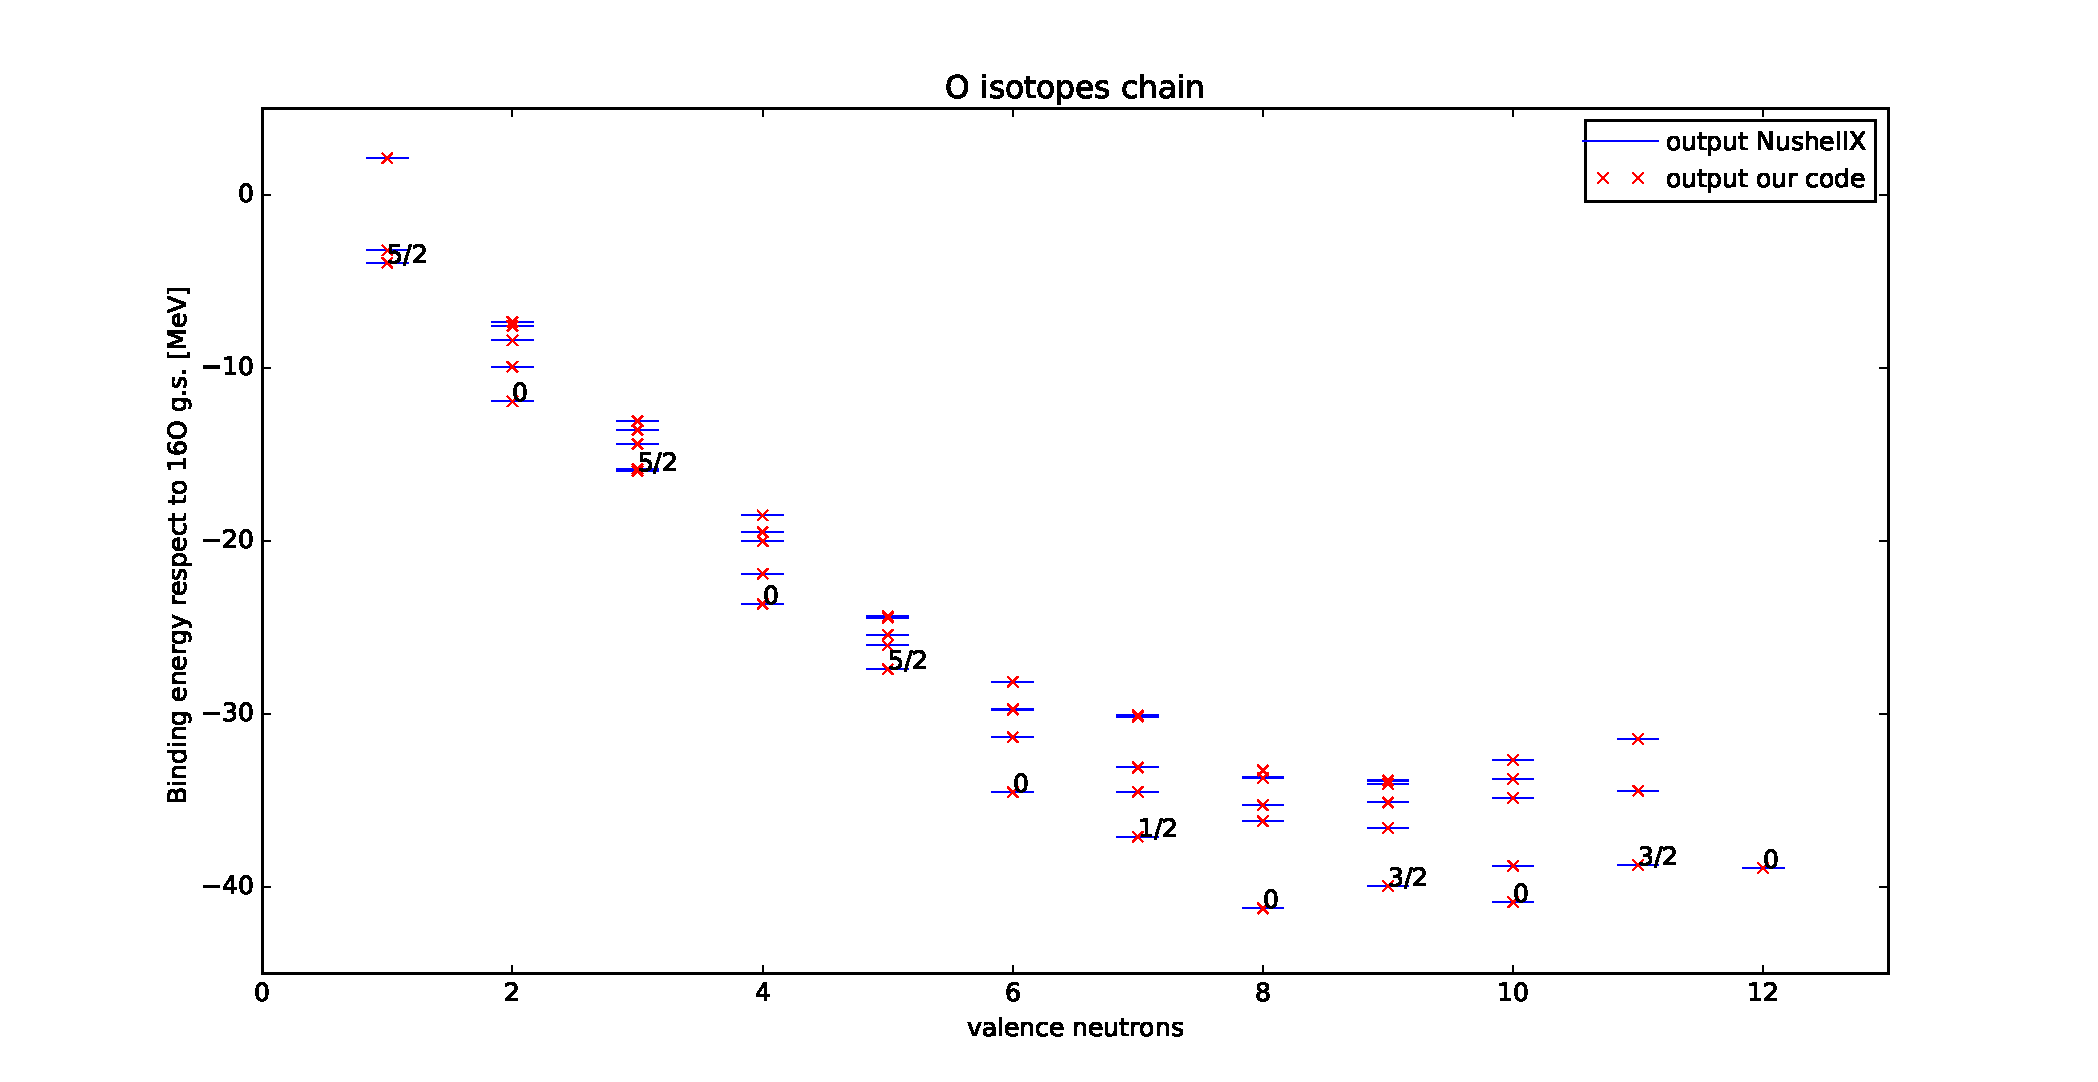
\includegraphics[width=1.\textwidth]{isotopes.pdf}
\caption{Comparison between NushellX and our code energy levels for the Oxygen isotopes. The $J$ value of the ground state is shown for each isotope}
\label{fig: isotopes}
\end{figure}

%[our shell-model results must go here. output in a listing or table? similar to what is in the 'Further considerations' chapter - move listing up here?] What kind of other results we want??? Ina: I meant to do exactly what you did (moved the listing above to this section and not have it where it was before).

%[also show results from the pairing model / unit test ? ] Gianluca: maybe no, they are already discussed in their Sec. Ina: I agree

%\begin{table}
%\caption{Example table}
%\centering
%\begin{tabular}{llr}
%\toprule
%\multicolumn{2}{c}{Name} \\
%\cmidrule(r){1-2}
%First name & Last Name & Grade \\
%\midrule
%John & Doe & $7.5$ \\
%Richard & Miles & $2$ \\
%\bottomrule
%\end{tabular}
%\end{table}


%------------------------------------------------
\newpage

\section{Discussion / Challenges and possible improvements}
\label{sec:discussion}

%[here we compare our code with NuShellX and comment other stuff (pairing model maybe).... ] Gianluca: already done before, here it is time for new things that can be interesting to implement or some remarks not made before


 %something about the accuracy of our code 
The numerical precision of the results can be crosschecked ut to KeV energies with NushellX. Since we are interested in energy levels, we consider that 1 KeV is enough because the main sources of theoretical 'errors' are the truncation of the model space and the values of the matrix elements fitted to reproduce the experimental states.

Instead a clear issue in this basic code is the time. Our code takes around 10s on a laptop to calculate the eigenvalues for 6 valence neutrons (the slowest possible calculation due to the largest possible number of Slater determinants). Among the total time 0.5s are required for the unit test, and the most of the time is spent in bulding the Hamiltonian matrix and diagonalize it. 
The calculating speed can be improved adopting an optimized diagonalization routine to replace the standard diagonalization done with numpy. Anyway to speed-up in a significative way we would need to introduce technique as the bit representation.

We spent a lot of time in debugging our sd-shell code. Future should use the tips given about debugging - could be implemented as unit tests? blah blah blah %Gianluca: I don't have anything to say here

%\subsection{Challenges and proposed solutions / Future work(?)}

The natural next step in the development of our code will be the introduction of valence protons in our model space. It will require some corrections to the body of the code, but we could increase our calculations until $^{40}$Ca (within the $sd$ model space).

An useful extension of our code will be to calculate the expectation value $\bra{\Psi_i} \hat J^2 \ket{\Psi_i}$ for each eigenstate $\ket{\Psi_i}$ of the Hamiltonian matrix, expressing the operator $\hat J^2$ in second quantization and applying Wick's theorem. In this way we could label each of the calculated energy levels with the relative total angular momentum.

If other than the total angular momentum we will implement in second quantization generic one-body operators we could calculate one-body transitions.

\section{Conclusions / Summary}
\label{sec:summary}

[here we have an amazing conclusion of our fabulous work and maybe summarize some stuff]


%----------------------------------------------------------------------------------------
%	REFERENCE LIST
%----------------------------------------------------------------------------------------

\begin{thebibliography}{99} 
% Bibliography - this is intentionally simple in this template
%
%\bibitem[Figueredo and Wolf, 2009]{Figueredo:2009dg}
%Figueredo, A.~J. and Wolf, P. S.~A. (2009).
%\newblock Assortative pairing and life history strategy - a cross-cultural
%  study.
%\newblock {\em Human Nature}, 20:317--330.
\bibitem[Github of the TALENT School][ MHJ and Alex Brown
\newblock {\em https://github.com/NuclearTalent/NuclearStructure}
%
\bibitem[NushellX]{ref: nushellx} 
\newblock {\em https://people.nscl.msu.edu/~brown/brown-all-papers/525-2014-nds120.115-nushellx.pdf}(and references within)
%
\bibitem[NushellX help]{help_file} 
\newblock {\em help/help.pdf}
%
\bibitem[usdb interaction file]{file_link}
\newblock {\em https://github.com/NuclearTalent/NuclearStructure/doc/pub/projects/datafiles/sdshellint.dat}
%
\bibitem[usdb 2006]{Brown 2006} B. Alex Brown and W. A. Richter,Phys. Rev. C \textbf{74} (2006) 034315
\newblock {\em https://journals.aps.org/prc/abstract/10.1103/PhysRevC.74.034315}
%
\end{thebibliography}

%----------------------------------------------------------------------------------------



%\section*{Structure of report (crude first idea):}
%
%\begin{enumerate}
%\item Title
%\item Abstract
%\item Introduction
%\begin{itemize}
%\item Why useful
%\item Where useful (nuc. chart)
%\item (Look at the TALENT proposal)
%\item comparing different tools
%\end{itemize}
%\item The Pairing problem
%\begin{itemize}
%\item theory
%\item analytic / exact results
%\end{itemize}
%\item Building a shell-model code
%\begin{itemize}
%\item Describe the different parts/blocks of the code (basis, SD, states, int, hamiltonian...)
%\item Unit tests / benchmarks (analytic/exact results)
%\item Psedo code?
%\item Accuracy of our code
%\item Where our code fails, why and proposing solutions
%\end{itemize}
%\item NuShellX
%\begin{itemize}
%\item describe why useful / 'powerful tool' and what may be calculated
%\item compare with our own code
%\item Possible 'future calculations'
%\end{itemize}
%\item Conclusions / Summary
%\end{enumerate}

%------------------------------------------------
%------------------------------------------------



\end{document}
